\documentclass[a4paper,12pt]{article}

\usepackage[brazil]{babel}
\usepackage{fontspec}
\usepackage{xeCJK}
\usepackage{xcolor}
\usepackage{ruby}
\usepackage{amsmath}
\usepackage{tcolorbox}
\usepackage{enumitem}
\usepackage{tabularx}
\usepackage{booktabs}

\setmainfont{Latin Modern Roman}
\setCJKmainfont{Noto Serif CJK JP}

\definecolor{jpnavy}{RGB}{20, 35, 60}
\definecolor{jpred}{RGB}{180, 40, 40}
\definecolor{lighthight}{RGB}{245, 247, 250}
\definecolor{jppurple}{RGB}{110, 70, 120}

\pagestyle{empty}

\begin{document}

\begin{center}
    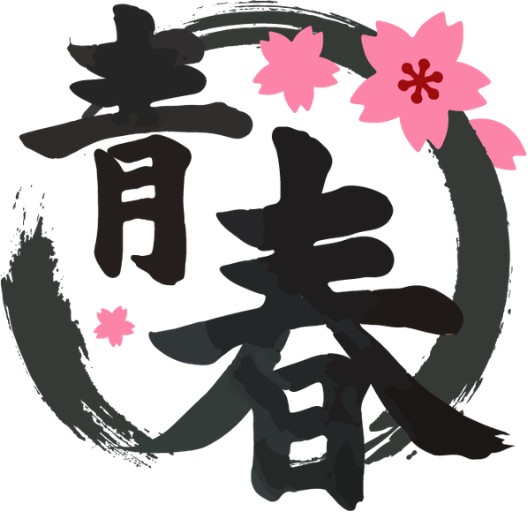
\includegraphics[height=2cm, keepaspectratio]{../Seishun.png}\\
    \vspace{0.3cm}
    {\LARGE\bfseries 第十三課}\\[4pt]
    \small オノマトペ (Onomatopeias)
\end{center}

\vspace{0.3cm}
\hrule height 1pt
\vspace{0.5cm}

\begin{tcolorbox}[colback=jppurple!6, colframe=jppurple, title=\textbf{Dica Cultural}, fonttitle=\bfseries]
\small
O japonês possui um dos sistemas de onomatopeias mais ricos do mundo, dividindo-se em três categorias principais:
\begin{itemize}[leftmargin=*, topsep=2pt, itemsep=1pt]
    \item \textbf{擬声語 (Giseigo):} Sons produzidos por vozes humanas e animais (ex: miados, risadas).
    \item \textbf{擬音語 (Giongo):} Sons de objetos inanimados e fenômenos da natureza (ex: chuva, vento, batidas).
    \item \textbf{擬態語 (Gitaigo):} Expressam estados físicos, condições emocionais, aspectos visuais ou ações silenciosas (ex: estar brilhando, andar preguiçosamente).
\end{itemize}
\textit{Nota de escrita:} Enquanto \textbf{Giseigo} e \textbf{Giongo} costumam ser escritos em \textbf{Katakana}, as expressões de estado (\textbf{Gitaigo}) aparecem com frequência em \textbf{Hiragana}.
\end{tcolorbox}

\vspace{0.2cm}

\subsection*{Tabelas de Onomatopeias Comuns}

\noindent
\small
\begin{tabularx}{\textwidth}{>{\bfseries\color{jppurple}}l X X}
\toprule
\multicolumn{3}{c}{\textbf{\color{jppurple}1. Sons de Animais e Vozes (擬声語 - Giseigo)}} \\
\midrule
Onomatopeia & Kana & Significado / Uso \\
\midrule
Nyaa-nyaa & ニャーニャー & Miado de gato \\
Wan-wan & ワンワン & Latido de cão \\
Piyo-piyo & ピヨピヨ & Piu-piu (pintinhos / pássaros pequenos) \\
Gero-gero & ゲロゲロ & Coachar de sapo \\
Kera-kera & ケラケラ & Risada alta / gargalhada descontraída \\
\midrule
\multicolumn{3}{c}{\textbf{\color{jppurple}2. Sons de Ações e Natureza (擬音語 - Giongo)}} \\
\midrule
Zaazaa & ザザー & Chuva forte / torrencial \\
Pota-pota & ポタポタ & Gotejar / pingos caindo \\
Doki-doki & ドキドキ & Batida forte do coração (nervosismo / empolgação) \\
Mogu-mogu & モグモグ & Mastigar de boca cheia \\
Paka-paka & パカパカ & Som de cascos de cavalo ao andar \\
\midrule
\multicolumn{3}{c}{\textbf{\color{jppurple}3. Estados, Sensações e Gestos (擬態語 - Gitaigo)}} \\
\midrule
Niko-niko & にこにこ & Sorriso radiante e silencioso \\
Kira-kira & きらきら & Brilhante / cintilante (estrelas, olhos) \\
Fuwafuwa & ふわふわ & Macio / fofinho (nuvens, algodão, bichos de pelúcia) \\
Peka-peka & ぺこぺこ & Com fome / estômago roncando \\
Goro-goro & ごろごろ & Ficar preguiçando em casa / rolar no chão \\
\bottomrule
\end{tabularx}

\newpage

\begin{center}
    {\LARGE\bfseries 会話 (História Infantil: O Urso e a Floresta)}
\end{center}

\textit{Cenário: Era uma vez um pequeno urso chamado Kuma-kun caminhando na floresta em um dia ensolarado, quando algo acontece...}

\vspace{0.8em}

\textbf{\ruby{語}{かた}り\ruby{手}{て}:} \ruby{晴}{は}れた\ruby{日}{ひ}、くまくんは\ruby{森}{もり}を\ruby{歩}{ある}いていました。お\ruby{腹}{はら}が\textbf{ぺこぺこ}です。\\
\textit{Katarite:} Hareta hi, Kuma-kun wa mori wo aruite imashita. O-hara ga \textbf{peko-peko} desu.\\
Narrador: Em um dia ensolarado, o pequeno urso estava caminhando pela floresta. Ele estava com muita fome!

\vspace{0.5em}

\textbf{くまくん:} あ、\ruby{空}{そら}に\ruby{星}{ほし}のようなものが\textbf{きらきら}ひかっているよ！なんだろう？\\
\textit{Kuma-kun:} A, sora ni hoshi no you na mono ga \textbf{kira-kira} hikatte iru yo! Nan darou?\\
Kuma-kun: Ah, tem algo brilhando no céu como uma estrela! O que será?

\vspace{0.5em}

\textbf{\ruby{小鳥}{ことり}:} \textbf{ピヨピヨ}！くまくん、こんにちは！あれはハチミツの\ruby{木}{き}だよ。\\
\textit{Kotori:} \textbf{Piyo-piyo}! Kuma-kun, konnichiwa! Are wa hachimitsu no ki da yo.\\
Pássaro: Piu-piu! Olá, Kuma-kun! Aquela é a árvore de mel.

\vspace{0.5em}

\textbf{くまくん:} わあ！ハチミツだ！\ruby{胸}{むね}が\textbf{ドキドキ}するよ！\\
\textit{Kuma-kun:} Waa! Hachimitsu da! Mune ga \textbf{doki-doki} suru yo!\\
Kuma-kun: Uau! É mel! Meu coração está batendo forte de emoção!

\vspace{0.5em}

\textbf{\ruby{語}{かた}り\ruby{手}{て}:} くまくんはハチミツを\textbf{モグモグ} \ruby{食}{た}べました。とても甘くて\ruby{美味}{おい}しいです。\\
\textit{Katarite:} Kuma-kun wa hachimitsu wo \textbf{mogu-mogu} tabemashita. Totemo amakute oishii desu.\\
Narrador: Kuma-kun mastigou o mel com gosto. Estava muito doce e delicioso!

\vspace{0.5em}

\textbf{くまくん:} \textbf{にこにこ}！お腹がいっぱいになったよ。\\
\textit{Kuma-kun:} \textbf{Niko-niko}! O-hara ga ippai ni natta yo.\\
Kuma-kun: (Sorrindo alegremente) Fiquei de barriga cheia!

\vspace{0.5em}

\textbf{\ruby{語}{かた}り\ruby{手}{て}:} すると、\ruby{突然}{とつぜん}\ruby{空}{そら}が\ruby{暗}{くら}くなり、\ruby{雨}{あめ}が\textbf{ザザー}と\ruby{降}{ふ}ってきました。\\
\textit{Katarite:} Suruto, totsuzen sora ga kuraku nari, ame ga \textbf{zaazaa} to futte kimashita.\\
Narrador: De repente, o céu escureceu e a chuva começou a cair bem forte!

\vspace{0.5em}

\textbf{くまくん:} うわあ、大変だ！\ruby{雨}{あめ}が\textbf{ポタポタ} \ruby{頭}{あたま}に\ruby{落}{お}ちてくる！\\
\textit{Kuma-kun:} Uwaa, taihen da! Ame ga \textbf{pota-pota} atama ni ochite kuru!\\
Kuma-kun: Nossa, que problema! As gotas de chuva estão pingando na minha cabeça!

\vspace{0.5em}

\textbf{\ruby{語}{かた}り\ruby{手}{て}:} くまくんは\ruby{大}{おお}きな\ruby{木}{き}の\ruby{下}{した}の\textbf{ふわふわ}なコケの\ruby{上}{うえ}で、\textbf{ごろごろ}しながら\ruby{雨}{あめ}やみを\ruby{待}{ま}ちました。\\
\textit{Katarite:} Kuma-kun wa oogisa na ki no shita no \textbf{fuwa-fuwa} na koke no ue de, \textbf{goro-goro} shina gara ameyami wo machimashita.\\
Narrador: Sob uma grande árvore, rolando confortavelmente sobre o musgo fofinho, o urso esperou a chuva passar.

\newpage

\subsection*{Vocabulário Útil (\textit{Tango})}

\vspace{0.2cm}

\noindent
\small
\begin{tabularx}{\textwidth}{>{\bfseries\color{jppurple}}l X X}
\toprule
Palavra (Romaji) & Kanji / Kana & Tradução em Português \\
\midrule
Doutobutsu & 動物 (どうぶつ) & Animal / Animais \\
Doubutsuen & 動物園 (どうぶつえん) & Zoológico \\
Mori & 森 (もり) & Floresta \\
Kotori & 小鳥 (ことり) & Passarinho \\
Inu & 犬 (いぬ) & Cão / Cachorro \\
Neko & 猫 (ねこ) & Gato \\
Usagi & 兎 (うさぎ) & Coelho \\
Kuma & 熊 (くま) & Urso \\
Zou & 象 (ぞう) & Elefante \\
Kirin & 麒麟 (きりん) & Girafa \\
Lion & ライオン & Leão \\
Panda & パンダ & Panda \\
Hachimitsu & ハチミツ & Mel \\
Ame & 雨 (あめ) & Chuva \\
Hikaru & 光る (ひかる) & Brilhar / Reluzir \\
O-hara ga ippai & お腹がいっぱい & Barriga cheia / Satisfeito \\
Koke & コケ & Musgo \\
\bottomrule
\end{tabularx}

\vspace{0.5cm}

\begin{tcolorbox}[colback=jppurple!6, colframe=jppurple, title=\textbf{Dinâmica em Grupo}, fonttitle=\bfseries]
\small
Escutar uma música chiclete japonesa para marcar o fim da primeira turma de japonês básico:

\vspace{0.2cm}

{\centering \Large\bfseries おしりフリフリ\par}
{\centering \small\textit{(Oshiri Furifuri --- Balançando o Bumbum)}\par}
\end{tcolorbox}

\vspace{0.4cm}

\begin{center}
    \small\color{gray} \textit{お疲れ様でした！}
\end{center}

\end{document}